% Copyright (c) 2013-2017 Christian Dietrich
%
% This work may be distributed and/or modified under the
% conditions of the LaTeX Project Public License, either version 1.3
% of this license or (at your option) any later version.
% The latest version of this license is in
%   http://www.latex-project.org/lppl.txt
% and version 1.3 or later is part of all distributions of LaTeX
% version 2005/12/01 or later.
%
% This work has the LPPL maintenance status `maintained'.
%
% The Current Maintainer of this work is Christian Dietrich
%
% This work consists of the files dataref.tex and dataref.sty

\documentclass{ltxdoc}
\usepackage[usagereport]{dataref}[2017/01/06]

\EnableCrossrefs
\CodelineIndex
\RecordChanges

\usepackage{verbatim}
\usepackage{listings}
\usepackage{pdfcomment}
\usepackage{siunitx}
\usepackage{xspace}
\usepackage{pgffor}
\usepackage{filecontents}
\usepackage{tikz}
\usetikzlibrary{positioning, arrows}

\begin{filecontents}{datapoints.tex}
\drefset{/control group/mice race}{Black Six}
\drefset{/control group/mice count}{32}
\drefset{/control group/dead after 24h}{4}
\drefset{/control group/dead after 48h}{7}
\drefset{/control group/recovered}{21}

\drefset{/med A/mice race}{Black Six}
\drefset{/med A/mice count}{32}
\drefset{/med A/dead after 24h}{6}
\drefset{/med A/dead after 48h}{12}
\drefset{/med A/recovered}{20}

\drefsethelp{.*/mice race}{The mice race used for experiments heavily
     influences the outcome of the results}

\drefsethelp{.*/(dead after|recovered)}{Of all infected mice, a
  certain number died within a specified period of time. A certain
  recovered from the infection. The dead categories are cumulative and
include all dead mice before.}
\end{filecontents}
\input{datapoints}
% \OnlyDescription
\drefkeys{prefix=/foo,value=123,save=/foo}
\drefset{/override test}{2}
\begin{document}
\drefsave{/override test}{4}
\drefkeys{prefix=}

\parskip=1ex
\parindent=0pt

\CheckSum{0}


 \CharacterTable
  {Upper-case    \A\B\C\D\E\F\G\H\I\J\K\L\M\N\O\P\Q\R\S\T\U\V\W\X\Y\Z
   Lower-case    \a\b\c\d\e\f\g\h\i\j\k\l\m\n\o\p\q\r\s\t\u\v\w\x\y\z
   Digits        \0\1\2\3\4\5\6\7\8\9
   Exclamation   \!     Double quote  \"     Hash (number) \#
   Dollar        \$     Percent       \%     Ampersand     \&
   Acute accent  \'     Left paren    \(     Right paren   \)
   Asterisk      \*     Plus          \+     Comma         \,
   Minus         \-     Point         \.     Solidus       \/
   Colon         \:     Semicolon     \;     Less than     \<
   Equals        \=     Greater than  \>     Question mark \?
   Commercial at \@     Left bracket  \[     Backslash     \\
   Right bracket \]     Circumflex    \^     Underscore    \_
   Grave accent  \`     Left brace    \{     Vertical bar  \|
   Right brace   \}     Tilde         \~}


 \changes{v0.6}{2016/11/15}{Units, Unit Scaling, general overhaul}
 \changes{v0.4}{2015/04/21}{Remove Spurious Whitespaces}
 \changes{v0.1}{2013/12/06}{Initial version}

 \DoNotIndex{\newcommand,\newenvironment}

 \makeatletter
 \def\colorfirsttoken#1#2{\bgroup\expandafter\color{#1}\cmd{#2}\egroup}
 \def\Macro@Name#1#2\@nnil{\string#1}

\renewcommand{\meta}[1]{\bgroup\color{green!40!black}$\langle$\textit{#1}$\rangle$\egroup}
\newcommand{\Macro}[2][]{%
  \noindent\hspace{-\marginparwidth}%
  \hypertarget{\Macro@Name#2\@nnil}{%
   \mbox{\colorfirsttoken{blue!50!black}#2}} \hfill\mbox{#1}\par}
 \newcommand{\Option}[2][]{%
   \noindent\hspace{-\marginparwidth}%
   \mbox{\color{red!50!black}#2} \hfill\mbox{#1}\par}

 \newcommand{\option}[1]{%
   \bgroup\color{red!50!black}#1\egroup\xspace
 }

 \renewcommand{\macro}[1]{%
   \hyperlink{\Macro@Name#1\@nnil}{\bgroup\color{blue!50!black}\cmd#1\egroup}\xspace
 }
 \makeatother

 \colorlet{examplefill}{yellow!80!black}
 \definecolor{codebackground}{rgb}{0.9,0.9,1}
 \newdimen\examplewidth
 \newsavebox{\codebox}
 \newenvironment{example}[1][\marginparwidth-12pt]
 {\begin{lrbox}{\codebox}\begin{minipage}{#1-2\fboxsep}}
 {\end{minipage}\end{lrbox}%
   \examplewidth=\wd\codebox%
   \addtolength{\examplewidth}{-\marginparwidth+15pt}%
   \global\examplewidth=\examplewidth%
  \noindent\hspace{-\marginparwidth}\colorbox{examplefill}{\usebox{\codebox}}\hspace{12pt}}

 \newenvironment{codeexample}
 {\begin{lrbox}{\codebox}\begin{minipage}{\textwidth-\examplewidth-2\fboxsep}}
{\end{minipage}\end{lrbox}\noindent\colorbox{codebackground}{\usebox{\codebox}}\global\examplewidth=0pt%
\par\vspace{1em}}%


 \newcommand{\dataref}{\textsc{dataref}\xspace}
 \providecommand*{\url}{\texttt}
 \GetFileInfo{dataref.sty}
 \title{The \textsf{dataref} package}
 \author{Christian Dietrich 2013-2016\\ \url{stettberger@dokucode.de}\\
        \url{https://github.com/stettberger/dataref}}
 \date{\filedate~\fileversion}

 \maketitle

 \section{Introduction}

 Writing scientific texts is a craft. It is the craft of communicating your results to your
 colleagues and to the curious world public. Often your conclusions are based upon facts and
 numbers that you gathered during your research for the specific topic. You might have done many
 experiments and produced lot of data. The craft of writing is to guide your reader through a
 narrative that is based upon that data. But there may be many versions of that data. Perhaps you
 found a problem in your experiment, while already writing, that forces you back into the
 laboratory. After a while, the moon has done its circle many times, you return from that dark
 place and your methodology has improved as significantly as your data has. But now you have to
 rewrite that parts of the data that reference the old data points.

 The \textsf{dataref} is here to help you with managing your data points. It provides you with
 macro style keys that represent symbolic names for your data points. You can reference those
 symbolic names with \macro{\dref}, use them in calculations to have always up-to-date percentage
 values, define projections between sets of data points and document them. \textsf{dataref} also
 introduces the notion of assertions (\macro{\drefassert}) for your results to ensure that your prosa
 text references fit the underlying data.

 \section{Usage (or \dref*{/control group/mice count} mice)}

 \begin{example}
   From the \dref{/med A/mice count} mice in the experiment, \drefcalc[prefix=/med A]{d(/mice
     count)-d(/recovered)} died.
 \end{example}
 \begin{codeexample}
   \verb|\drefset{/med A/mice count}{32}|\\
   \verb|\drefset{/med A/recovered}{20}|\\
   \verb|From the \dref{/med A/mice count} mice in the experiment, |\\
   \verb|\drefcalc[prefix=/med A]{d(/mice count)-d(/recovered)} died.|
 \end{codeexample}

 \subsection{Design Principles}

 Before we jump into the description of \dataref, let us look a little bit into the design principles of \dataref. By
 understanding the principles, you will be more productive and embedding data into your document will become easier.

 First of all, \dataref is built on top of \textsf{pgfkeys} and \textsf{pgfmath} from the PGF/TiKZ macro packages. While
 the former provides a usable user interface to provide options to \dataref, the later is used to perform computation on
 your datapoints. If you are interested into these two excellent \TeX{} packages, please look at \texttt{texdoc
   pgfmanual} for further information.

 There are two aspects of \dataref: setting datapoints and referencing datapoints. While setting datapoints is kind of
 boring, we have a wide variety of options when it comes to referencing. The expansion of datapoints is done in
 multiples phases (see Figure~\ref{fig:pipeline}).


 \begin{figure}[t]
  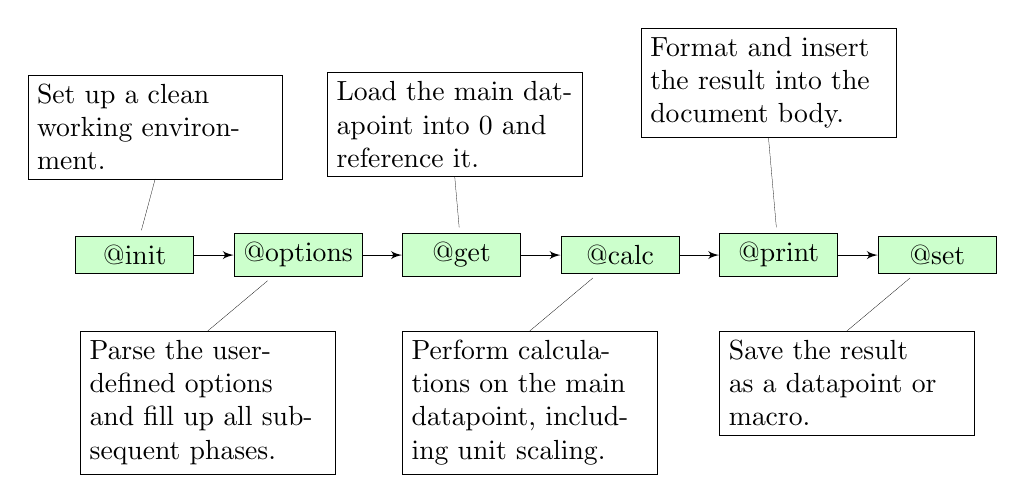
\begin{tikzpicture}[node distance=0.5cm]
    \tikzstyle{phase}=[draw,minimum width=1.5cm, fill=green!20!white];
    \tikzstyle{desc}=[align=left, text width=3cm,anchor=#1,draw];


   \node[phase](@init){@init};
   \node[phase,right=of @init](@options){@options};
   \node[phase,right=of @options](@get){@get};
   \node[phase,right=of @get](@calc){@calc};
   \node[phase,right=of @calc](@print){@print};
   \node[phase,right=of @print](@set){@set};

   \draw[>=latex']
     (@init) edge[->] (@options)
     (@options) edge[->] (@get)
     (@get) edge[->] (@calc)
     (@calc) edge[->] (@print)
     (@print) edge[->] (@set);

     \draw[ultra thin,shorten <=2pt] (@init) -- ++(75:1cm)
        node[desc=south] {Set up a clean working environment.};

      \draw[ultra thin,shorten <=2pt] (@options) -- ++(-140:1.5cm)
        node[desc=north] {Parse the user-defined options and fill up all subsequent phases.};

      \draw[ultra thin,shorten <=2pt] (@get) -- ++(95:1cm)
        node[desc=south] {Load the main datapoint into \macro{\drefresult} and reference it.};

      \draw[ultra thin,shorten <=2pt] (@calc) -- ++(-140:1.5cm)
       node[desc=north] {Perform calculations on the main datapoint, including unit scaling.};

      \draw[ultra thin,shorten <=2pt] (@print) -- ++(95:1.5cm)
        node[desc=south] {Format and insert the result into the document body.};

      \draw[ultra thin,shorten <=2pt] (@set) -- ++(-140:1.5cm)
       node[desc=north] {Save the result as a datapoint or macro.};

     \end{tikzpicture}
     \caption{The \dataref Pipeline}\label{fig:pipeline}
   \end{figure}

   The \dataref macros are different regarding the phases they include or omit and in their default settings. In the
   following, we will discuss all options and macros you can use to reference your datapoints. By default, the
   \macro{\drefresult} is always set to the result of the pipeline.

 \subsection{Setting Datapoints}



 \Macro[(@set)]{\drefset\oarg{options}\{\meta{name}\}\{\meta{value}\}}


\begin{codeexample}
\begin{verbatim}
\drefset{/med A/mice race}{Black Six}
\drefset{/med A/mice count}{32}
\drefset{/med A/dead after 24h}{6}
\drefset{/med A/dead after 48h}{1}
\end{verbatim}
\end{codeexample}


 The \macro{\drefset} command is used to define the symbolic datapoints. The name of a datapoint may contain virtually all
 characters, including spaces and slashes. It is good practice to use a hierarchy to structure your data point names.
 The value might be any string, while the focus of \dataref is on numerical datapoints. The \macro{\drefset} command works
 outside the pipeline model (Figure \ref{fig:pipeline}) for performance reasons. It virtually consists only of the
 @options and @set stage.

 \Macro[(@set)]{\drefsave[\meta{options}]\{\meta{name}\}\{\meta{value}\}}

 Besides setting the datapoint, \macro{\drefsave} writes it to the \textsc{aux} file and, therefore, makes it available in
 the next \LaTeX{} run from the very beginning. The \option{ignoremissing} option is useful to reference the saved keys
 at an earlier place in the document.

\Option[(no default)]{/dref/set=\meta{key}}

Inserts a \macro{\drefset} to the @set that captures the current result and saves it to the given datapoint.

\Option[(no default)]{/dref/save=\meta{key}}

Inserts a \macro{\drefsave} to the @set that captures the current result and saves it to the given datapoint. Since
\macro{\drefsave} is used the result is available from the beginning of the document.

\Option[(no default)]{/dref/to macro=\meta{macro}}

The current result is saved to the given macro.

\begin{example}[2cm]
  \dref[set=/foo]{/med A/mice count} \dref{/foo}\\
  \dref[ignoremissing]{/bar} \dref[save=/bar]{/med A/mice count}\\
  \drefcalc*[to macro=\myresult]{3+2} \myresult
\end{example}
\begin{codeexample}
\begin{verbatim}
\dref[set=/foo]{/med A/mice count} \dref{/foo}\\
\dref[ignoremissing]{/bar} \dref[save=/bar]{/med A/mice count}\\
\drefcalc*[to macro=\myresult]{3+2} \myresult
\end{verbatim}
\end{codeexample}


\Option[(no default, initially "")]{/dref/prefix=\meta{key prefix}}

On every key retrieval or setting of a datapoint this prefix is added.
It is a value-typed PGF key, so operations like
\texttt{prefix/.append} are possible.

\Macro{\drefinput[\meta{prefix}]\{\meta{filename}\}}

Reads in the given \TeX/dataref file with the given key prefix. Therefore, all included \cmd{\drefset} commands are define their keys with the given prefix.
This is useful to include several files that resulted from different experiments but include equal datapoint keys.

This command uses \cmd{\subimport} from the \texttt{import} package to read the file.
Hence, if there is an \cmd{\drefinput} in an included file, it search its filename relative to its own directory.\footnote{In former versions, \cmd{\drefinput} relied directly on \cmd{\input} and, therefore, the filename was interpreted relative to the root file.}.


\subsection{Referencing Datapoints}


 \Macro[(@options=\{print=default\}, @get, @calc, @print, @set)]{\dref*[\meta{options}]\{\meta{name}\}}
 \Macro[(@options=\{print=raw\},     @get, @calc, @print, @set)]{\dref[\meta{options}]\{\meta{name}\}}

 This macro is used to reference a single symbolic data point. The value stored in that datapoint is inserted into the
 text. \macro{\dref} additionally marks the data point as used; it will appear in the datagraphy (see
 Section~\ref{sec:datagraphy}). The starred variant does not attempt to parse the datapoint as a numerical value, but
 outputs the saved string.

\begin{example}
\dref*{/control group/mice race}\\
\dref*{/control group/mice count}\\
\dref[sci,precision=2,zerofill=true]{/med A/recovered}
\end{example}
\begin{codeexample}
\begin{verbatim}
\dref*{/control group/mice race}\\
\dref*{/control group/mice count}\\
\dref[sci,precision=2,zerofill=true]{/med A/recovered}
\end{verbatim}
\end{codeexample}

\Macro[(@get, @print)]{\drefvalueof\{\meta{name}\}}
\Macro[(@get)]{\drefref\{\meta{name}\}}
\vspace{1em}

\begin{example}
\drefvalueof{/med A/mice race}
\end{example}\begin{codeexample}
\begin{verbatim}
\drefvalueof{/med A/mice race}
\end{verbatim}
\end{codeexample}

  Since \macro{\dref} is not expandable, it cannot be used in all circumstances. Therefore, \macro{\drefvalueof} bypasses
  all internal bookkeeping and provides access to the raw datapoint value. \macro{\drefref} can be used to mark the
  datapoint as used to let it appear in the datagraphy.

\Option[(default \textbf{true}, initially \textbf{false})]{/dref/ignoremissing=\meta{true-or-false}}
\Option[(no default, initially \textbf{1.0})]{/dref/defaultvalue=\meta{value}}

By default, \dataref produces an error if the referenced datapoint is undefined. If ignoremissing is given, the
defaultvalue is used. This key is useful in combination with \macro{\drefsave}. Furthermore, it is possible to extract the
missing keys from the \textsc{aux} file and to retrieve it from a secondary source (e.g. database, wikidata, etc).

\begin{example}
\dref*[ignoremissing,defaultvalue=undefined]{blah}
\end{example}\begin{codeexample}
\begin{verbatim}
\dref*[ignoremissing,defaultvalue=undefined]{blah}
\end{verbatim}
\end{codeexample}

\Macro{\drefsethelp\{\meta{pattern}\}\{\meta{text}\}}
\Macro{\drefhelp\{\meta{name}\}}

 \textsf{dataref} comes with a simple method for defining documentation for data points. This help can for example be used to communicate what is the concrete semantics of the data point. This is of special interest when writter and data gatherer are not the same person. \macro{\drefsethelp} takes two arguments: first a regular expression that matches the symbolic data point, second the help text.

\begin{codeexample}
\begin{verbatim}
\drefsethelp{.*/mice race}{The mice race used for experiments
 heavily influences the outcome of the results}
\end{verbatim}
\end{codeexample}

The documentation for a datapoint is obtained by using the \macro{\drefhelp} macro. It checks all defined documentation
strings (in linear order, first defined, first matched), and prints the first matching help text. With \textbf{LuaTeX}:
only Lua (string.find) regular expressions are supported as patterns.

 \begin{example}
    \drefhelp{/med A/mice race}
  \end{example}\begin{codeexample}
\begin{verbatim}
\drefhelp{/med A/mice race}
\end{verbatim}
  \end{codeexample}


\Macro{\drefresult}

Is set in the @set phase to the result of the currently executed pipeline.


\subsection{Calculations and Math Tools}

\Macro[(@calc, @print, @set)]{\drefcalc[\meta{options}]\{\meta{expression}\}}
\Macro[(@calc, @set)]{\drefcalc*[\meta{options}]\{\meta{expression}\}}
\Macro[(@print)]{\drefformat*[\meta{options}]\{\meta{number}\}}

The \macro{\drefcalc} is the core function of calculating with data points. It is based on the pgfmath engine, but allows
also the usage of symbolic datapoints within mathematical expressions. Datapoints can either are inserted into the
calculations with the \cmd{d(\meta{path})} or the \cmd{data("\meta{path}")} notation. The starred variant of
\macro{\drefcalc} does not print the result, but only sets the result macros.

It is important to note, that \macro{\drefcalc} always uses the \textbf{/pgf/fpu} environment. The FPU feature of pgfmath
is used to handle large numbers, which may occur often when handling experiment data points.

\begin{example}
  \drefcalc{(4+7)/12 * 100}\\
  \drefcalc{d(/med A/mice count) * 100}\\
  \drefcalc{data("/med A/mice count") * 100}\\
  \drefcalc*{1+3}\\
  \drefresult
\end{example}\begin{codeexample}
\begin{verbatim}
\drefcalc{(4+7)/12 * 100}\\
\drefcalc{d(/med A/mice count) * 100}\\
\drefcalc{data("/med A/mice count") * 100}\\
\drefcalc*{1+3}\\
\drefresult
\end{verbatim}
\end{codeexample}

Since the default printing mechanism of \dataref utilizes PGF, all options from \texttt{/pgf/number format} can be
directly used in the options. \macro{\drefformat} does only the printing. For documentation on the available options,
please consult the PGF manual.

\begin{example}
  \drefcalc[precision=4]{1/3}\\
  \drefcalc[sci]{123456789}\\
  \drefcalc[prefix=/med A/,frac]{d(recovered)/d(mice count)}\\
  \drefformat[fixed zerofill, precision=2]{\drefresult}
\end{example}\begin{codeexample}
\begin{verbatim}
\drefcalc[precision=4]{1/3}\\
\drefcalc[sci]{123456789}\\
\drefcalc[prefix=/med A/,frac]{d(recovered)/d(mice count)}\\
\drefformat[fixed zerofill, precision=2]{\drefresult}
\end{verbatim}
\end{codeexample}

\subsection{Units and Unit Scaling}

\dataref allows to give the unit of a datapoint and enforces the correct combination of units when using them in
calculations. \dataref units can be arbitrary combinations of macros and strings, which allows the combination with the
\textsc{SIUnitX} package.

\Option[(no default)]{/dref/unit=\meta{unit}}

The unit of a datapoint is loaded in the @get phase, and stored in the @set phase of the \dataref pipeline.

\drefset[unit=\joule]{/power}{1234}
\drefset[unit=ms]{/duration}{5555}
\begin{codeexample}
\begin{verbatim}
\drefset[unit=ms]{/duration}{5555}
\drefset[unit=\joule]{/power}{1234}
\end{verbatim}
\end{codeexample}

\Option[(no default, choice)]{/dref/unit/format=\meta{formatting style}}
\Option[(initially \textbf{plain})]{/dref/unit/format default=\meta{formatting style}}


If a datapoint with unit is referenced, the unit is printed after the value. The formatting mechanism can be exchanged,
in order to omit the unit, or to use \textsc{SIUnitX} for properly print it. By default, the \texttt{unit/format
  default} is set in the @init phase. If you are using \textsc{SIUnitX} in your document, it is safe to set the default
value accordingly. Currently, the values \texttt{false}, \texttt{plain}, and \texttt{siunitx} are valid formatting
styles.

\drefkeys{unit/format default=siunitx}
\begin{example}
  \dref[unit/format=false]{/duration}; \dref{/duration};
    \typeout{\pgfkeysvalueof{/dref/unit/format default}}
    \dref{/power}
\end{example}\begin{codeexample}
\begin{verbatim}
\drefkeys{unit/format default=siunitx}
\dref[unit/format=false]{/duration}; \dref{/duration};
\dref{/power}
\end{verbatim}
\end{codeexample}

\Option[(no default)]{/dref/unit/new scala=\meta{scala}}

\dataref allows to define scaled units and conversion between the members of the scala. A scala definition is a list of
units with scaling factors between them.


\drefkeys{
  unit/new scala={
    1/y, 365/d, 24/h, 60/m, 60/s, 1000/ms, 1000/us, 1000/ns
  },
  unit/new scala={
    1/\kilo\joule, 1000/\joule, 1000/\milli\joule,
    1000/\micro\joule, 1000/\nano\joule
  }
}

\begin{codeexample}
\begin{verbatim}
\drefkeys{
  unit/new scala={
    1/y, 365/d, 24/h, 60/m, 60/s, 1000/ms, 1000/us, 1000/ns
  },
  unit/new scala={
    1/\kilo\joule, 1000/\joule, 1000/\milli\joule,
    1000/\micro\joule, 1000/\nano\joule
  }
}
\end{verbatim}
\end{codeexample}

\Option[(no default)]{/dref/unit/scale to=\meta{unit}}

With a defined scala, you can scale to any unit on that scala automatically. In the example, we use unit to set the unit
of plain value to nano joule, and scale everything to milli joule.

\begin{example}
\foreach \a in {1234, 4135413, 213516513245, 24} {%
  \drefformat[unit=\nano\joule, unit/scale to=\milli\joule]{\a}\\
}
\end{example}\begin{codeexample}
\begin{verbatim}
\foreach \x in {1234, 4135413, 213516513245, 24} {%
  \drefformat[
    unit=\nano\joule,
    unit/scale to=\milli\joule]{\x}\\
}
\end{verbatim}
\end{codeexample}

\Option[(default \textbf 50)]{/dref/unit/scale to auto=\meta{optimum number}}

With \texttt{scale to auto}, the appropriate unit is chosen automatically. The algorithm tries every unit on the scala
and chooses the unit, where the numerical value after scaling is nearest to the \meta{optimum number}. So with a optimum
number of 50, 5000 seconds are scaled to \drefformat[unit=s, unit/scale to auto]{5000} instead of \drefformat[unit=s,
unit/scale to=h]{5000}.


\begin{example}
\foreach \a in {1234, 4135413, 213516513245, 24} {%
  \drefformat[unit=ms, unit/scale to auto]{\a}\\
}
\end{example}\begin{codeexample}
\begin{verbatim}
\foreach \x in {1234, 4135413, 213516513245, 24} {%
  \drefformat[unit=ms, unit/scale to auto]{\x}\\
}
\end{verbatim}
\end{codeexample}


\subsection{Relating Datapoints}

\Macro[(@calc, @set)]{\drefrel*[\meta{options}]\{\meta{key or value}\}}
\Macro[(@calc, @print, @set)]{\drefrel[\meta{options}]\{\meta{key or value}\}}

Often, datapoints are set in relation to each other. This can either be done with \macro{\drefcalc} or, more explictily,
with \macro{\drefrel}. The different options that come along \macro{\drefrel}, add steps to the @calc phase and can,
therefore, be combinated with any other dref macro that includes the @calc phase.

All operations operate on the current result, which is initially the given key or value from the mandatory argument.

\begin{example}
  \drefrel[percent of=123]{40}
\end{example}\begin{codeexample}
\begin{verbatim}
  \drefrel[percent of=123]{40}
\end{verbatim}
\end{codeexample}

The different relation operations try to have a speaking name, such that the \TeX{} code is easily understandable by the
writer. This explicit notation aims to prevent common mistakes, like confusing denominator and numerator.

The starred version of \macro\drefrel does not print any number, but only saves the result in \macro\drefresult. Instead of
only taking datapoint keys, \macro\drefrel, as well as the relating operations, take either a key or a bare number as you can
see from the example.

\Option[(no default)]{/dref/scale by=\meta{key or value}}

Scales the current value by the given factor, which must be unit less. The resulting unit is untouched.

\Option[(no default)]{/dref/percent}

Scales the current value by 100. The unit is not changed.

\Option[(no default)]{/dref/negate}

Scales the current value by -1. The resulting unit is untouched.

\Option[(no default)]{/dref/divide by=\meta{key or value}}

Divides the current value by the given factor, which must be unit less. The resulting unit is untouched.


\Option[(no default)]{/dref/abs}

Calculate the absolute value.

\Option[(no default)]{/dref/factor of=\meta{key or value}}
\Option[(no default)]{/dref/percent of=\meta{key or value}}

The \textbf{factor of} operation gives the portion the current value in relation to the given base value. In easy words:
a division. This macro ensures, that base and current vale have the same unit or are unit less. The result of this
operation is unit less. The \textbf{percent of} operation, furthermore, scales the result with 100 to get a percentage.

\Option[(no default)]{/dref/increase from=\meta{key or value}}
\Option[(no default)]{/dref/decrease from=\meta{key or value}}
\Option[(no default)]{/dref/increase factor from=\meta{key or value}}
\Option[(no default)]{/dref/decrease factor from=\meta{key or value}}
\Option[(no default)]{/dref/increase percent from=\meta{key or value}}
\Option[(no default)]{/dref/decrease percent from=\meta{key or value}}

In a situation, where a datapoint is the result of a changed experiment setup, the value normally shows an increased or decrease
numerical value. This family of operations calculates this delta, assuming it is an increase or decrease. The factor
operations scale the result to the base value, and the percent operations give this scaled value as a percentage.

\begin{example}
  \drefrel[increase from=500]{525}\\
  \drefrel[increase factor from=500,fixed]{525}\\
  \drefrel[increase percent from=500]{525}\,\%
\end{example}
\begin{codeexample}
\begin{verbatim}
  \drefrel[increase from=500]{525}\\
  \drefrel[increase factor from=500,fixed]{525}\\
  \drefrel[increase percent from=500]{525}\,\%
\end{verbatim}
\end{codeexample}

\subsection{Helper Utilities}

\Macro{\drefrow[\meta{options}]\{\meta{comma-separated list}\}\{\meta{key template}\}}
\Macro{\drefrow*\{\meta{comma-separated list}\}\{\meta{template}\}}

 Often different columns in a table have to be obtained from your data
 points. Often those rows and columns are similar. Generating parts of
 tables within \LaTeX is very tricky, so \dataref provides you
 with \macro{\drefrow}. This macro iterates over a comma-separated list
 of values and fills out a macro which is interpreted as a symbolic
 data point. The entries are seperated with \& and printed. In the
 starred variant the resulting text is not interpreted as symbolic
 name, but as a macro.

 Both, unstarred and starred variant take a template (a macro body) that is expanded once for every item in the given
 list. The first replacement \verb|#1| is list item and the second \verb|#2| is the current index starting from 0. The
 unstarred variant interprets the expanded result as a datapoint key and uses \macro\dref to expand it; the optional
 parameter is passed through to every invocation of \macro\dref.
 The starred variant does not wrap the result into \macro\dref, and, therefore, is more flexible.

 \begin{example}
   \begin{tabular}{|c|c|c|}\hline
   \drefrow{dead after 24h,dead after 48h,recovered}%
                           {/control group/#1}\\\hline
   \drefrow{dead after 24h,dead after 48h,recovered}%
                           {/med A/#1}\\\hline
   \end{tabular}
 \end{example}
 \begin{codeexample}
\begin{verbatim}
\begin{tabular}{|c|c|c|}\hline
  \drefrow{dead after 24h,dead after 48h,recovered}
           {/control group/#1}\\\hline
  \drefrow{dead after 24h,dead after 48h,recovered}%
          {/med A/#1}\\\hline
\end{tabular}
\end{verbatim}
 \end{codeexample}


 \Macro[(@calc)]{\drefassert\{\meta{expr}\}}

 Sometimes the underlying data changes while you are writing. But what
 if your prose text relies on certain characteristics of the data. \macro{\drefassert} uses a pgfmath
 expression that evaluates to \verb|true| or \verb|false|. When the
 assertion holds (\verb|true|) nothing happens, only a terminal message
 is printed. When it does not hold (\verb|false|) the compilation is aborted.

\begin{example}
\drefassert{data("/control group/mice count") > 30}
Of the more than thirty infected mice...
\end{example}\begin{codeexample}
\begin{verbatim}
\drefassert{data("/control group/mice count") > 30}
Of the more than thirty infected mice...
\end{verbatim}
\end{codeexample}

 \Option[(default \textbf{true})]{/dref/noassert=\meta{true or false}}

 The \textbf{noassert} deescalates all assertion errors to mere warnings. This option can also be given at the
 \cmd{\usepackage} invication.

\Option[(no default, initially \textbf{none}, choice)]{/dref/annotate=\meta{annotation type}}
\Option[(choice item)]{/dref/annotate=none}
\Option[(choice item)]{/dref/annotate=footnote}
\Option[(choice item)]{/dref/annotate=pdfcomment}
\Option[(choice item)]{/dref/annotate=typeout}

While writing a document it is desirable to know, what key is used, while writing the text and generating the document.
Therefore \dataref provides the possibility to annotate values. The default option \textbf{none} disables this kind of
annotation. The \textbf{pdfcomment} option uses pdf annotations. Be aware that those annotations work properlyy only on
a few selected PDF readers\footnote{In doubt use Acrobat}.

\begin{example}[6cm]
  \drefkeys{annotate=footnote}
  \dref*{/control group/mice race}
  \dref{/control group/mice count}
  \drefcalc[annotate=pdfcomment]{100/3}
\end{example}\begin{codeexample}
\begin{verbatim}
\drefkeys{annotate=footnote}
\dref*{/control group/mice race}
\dref{/control group/mice count}
\drefcalc[annotate=pdfcomment]{100/3}
\end{verbatim}
\end{codeexample}


 \subsection{Datagraphy}\label{sec:datagraphy}

 \Macro{\drefusagereport}
 \Option{[usagereport]}
 \Option{[refall]}

 With the \textbf{usagereport} package option enabled, \macro{\drefusagereport} generates a usagereport of all referenced
 keys. The usage report groups the keys by the help texts. If the refall package option is given, all keys are marked as
 referenced.

\section*{Datagraphy}
\drefusagereport

\end{document}

%%% Local Variables:
%%% mode: latex
%%% TeX-master: t
%%% End:
